\documentclass[12pt]{amsart}

\theoremstyle{plain}
\newtheorem{theorem}{Theorem}
\newtheorem{lemma}[theorem]{Lemma} 
\newtheorem{conjecture}[theorem]{Conjecture} 
\newtheorem{corollary}[theorem]{Corollary}
\newtheorem{proposition}[theorem]{Proposition}
\theoremstyle{definition}
\newtheorem{definition}[theorem]{Definition}

\usepackage{fullpage,hyperref,url}
\usepackage[pdftex]{graphicx}

\title{Project Draft: Quintic Spectrahedra}
\author{Jacob Emmert-Aronson}
\author{Moor Xu}
\date{April 16, 2014}
\begin{document} 
\maketitle

\emph{Spectrahedra} of degree $n$ in $\mathbb{R}^k$ are convex bodies
given by $k$-dimensional affine slices of the cone of $n \times n$
positive semidefinite matrices.  They arise as feasible domains in
semidefinite programming and each is described by a linear matrix
inequality.
\vspace\baselineskip

\begin{center}

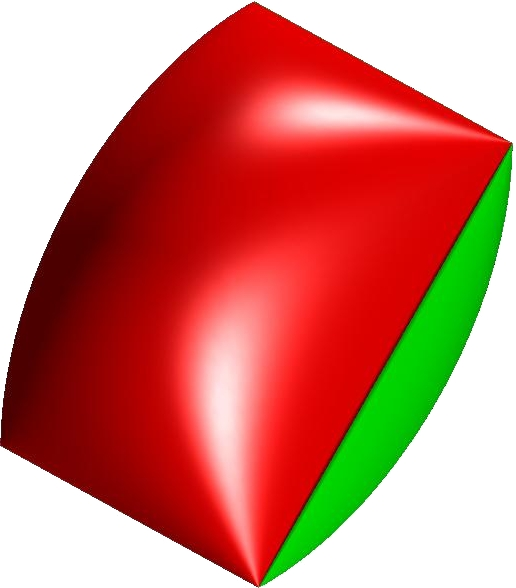
\includegraphics[scale=.15]{pillow.jpg}
\vspace\baselineskip

{\small
\emph{The pillow}: the spectrahedron
$
\begin{pmatrix}
  1&x&0&x\\
  x&1&y&0\\
  0&y&1&z\\
  x&0&z&1
\end{pmatrix}
\succeq 0\text.$  Here $k=3,\, n=4$.}
\end{center}
\vspace\baselineskip

Because the cost function of an SDP is linear, the optimal point
always lies on the surface.  One interesting and practically useful
question is the likelihood for the result of an optimization to be a
node, one of the corner points seen when visualizing the
spectrahedron.  A generic matrix represented by a point on the surface
of the spectrahedron has rank $n-1$, while the matrix at a node
typically has rank $n-2$.  This low-rank property of nodes often
translates to easier computation.

It is important to understand the nodal structure of a spectrahedron. 
This structure is well-understood in the quartic case. 
\cite{OKSV} classifies the number of nodes that quartic spectrahedra can have. 
\begin{theorem}\label{quartic}
	There exists a quartic spectrahedron with $\sigma$ nodes on its boundary and
	$\rho$ real nodes in its symmetroid if and only if $0 \le \sigma \le \rho$,
	both are even, and $2 \le \rho \le 10$.
\end{theorem} 
We studied the nodal structure of quintic spectrahedra in hopes of obtaining an
analogous result.

To carry this out, we generated random spectrahedra and computed
the positions of nodes, while also running multiple optimization
problems on each.  Jacob Emmert-Aronson and Joe Kileel wrote much of
the code to carry this out last semester.  
We had used Singular
to determine locations of nodes through a Gr\"obner basis algorithm;
due to apparent numeric instabilities, however, this misidentified
nodes in certain edge cases.  We have replaced this with the
homotopy algorithms implemented in Bertini, which have produced more
reliable results.  

We are now generating a new data set to determine possible node counts with
relative frequencies, and other properties which may be of interest.  After
generating 6723 random quintic spectrahedra and computing their nodes, we have
observed the following behavior. Here, $\sigma$ is the number of nodes on the
boundary of the spectrahedra, $\rho$ is the number of real nodes in its
symmetroid, and $p$ is the probability of observing these node counts upon
generating a random quintic spectrahedron. (Some node counts occurred with
very low probability.)

\begin{center}
\begin{tabular}{| l | l | l |} 
	$\sigma$ & $\rho$ & $p$ \\ \hline
	0 & 4 & 0.002    \\
	0 & 6 & 0.002    \\
	0 & 8 & low    \\
	0 & 10 & low    \\
	2 & 2 & low    \\
	2 & 4 & 0.010    \\
	2 & 6 & 0.061    \\
	2 & 8 & 0.075    \\
	2 & 10 & 0.028    \\
	2 & 12 & 0.005    \\
	2 & 14 & 0.001    \\
	4 & 4 & low    \\
	4 & 6 & 0.023    \\
	4 & 8 & 0.153    \\
	4 & 10 & 0.236    \\
	4 & 12 & 0.096    \\
	4 & 14 & 0.021    \\
	4 & 16 & 0.003    \\
	6 & 6 & low    \\
	6 & 8 & 0.009    \\
	6 & 10 & 0.065    \\
	6 & 12 & 0.114    \\
	6 & 14 & 0.056    \\
	6 & 16 & 0.013    \\
	6 & 18 & 0.001    \\
	8 & 10 & 0.001    \\
	8 & 12 & 0.005    \\
	8 & 14 & 0.011    \\ \hline
\end{tabular} 
\end{center}

We believe that with more data, we will see more types of quintic spectrahedra,
and we conjecture that a result analogous to Theorem \ref{quartic} holds in the
quintic case. This requires some further study.


%%%%%%%%%%%%%%%%%%%%%%%
\bibliographystyle{amsplain}
\bibliography{references}
\nocite{*}

\end{document} 


